\part{Resultados}

\chapter[Resultados]{Resultados}\label{Capitulo5}

Este trabalho resultou em uma aplicação Web que melhora a comunicação na fase interna de licitação, contribuindo para alcançar o princípio constitucional da eficência.
Essas melhorias foram atingidas mapeando os problemas através do levantamento de requisitos e em seguida desenvolvendo soluções representadas inicialmente em casos de uso posteriormente implementados.
A solução permite que entes de um mesmo órgão da administração pública federal comuniquem-se durante a fase interna da licitação.
Essa comunicação ocorre para maximizar o número de itens em uma compra e minimizar a quantidade de procesos licitatórios com itens repetidos.

Além disso, a solução abrange um banco de dados com informações sobre itens, materiais, serviços e licitações, fornecendo ao usuário informações atualizadas sobre processos licitatórios.
A obtenção desses dados é feita através de ação no sistema que recupera os dados na API de Compras Governamentais, forma pela qual o banco de dados pode se manter sempre atualizado com as licitações mais recentes.
O banco de dados que pode ser atualizado automaticamente mediante ação do usuário, com um clique em um botão atualizar.

A sequência de figuras apresentada a seguir, demonstra o processo de comunicação entre entes da administração pública federal durante a fase interna, para a compra de um \textit{selo de segurança}.
Uma vez que um ente ``A'' inicia um processo licitatório para a compra do selo, ele comunica outros entes da rede sobre sua intenção  com um prazo de adesão definido.
Se um ente ``B'' da rede, também tem intenção de comprar o mesmo item, ele acrescenta a quantidade desejada ao processo já iniciado, respeitando o prazo de adesão.

A Figura~\ref{tela01} apresenta a tela inicial do sistema.
A Figura~\ref{tela02} apresenta a requisição que cada ente recebe após iniciado um processo licitatório.
A Figura~\ref{tela03} mostra como um ente ``B'' pode aderir ao processo licitatório iniciado, inserindo sua demanda para os itens apresentados.
A Figura~\ref{tela04} apresenta a resposta  à requisição do ente ``B'' para o ente ``A''.
\begin{figure}[htp]
	\centering
	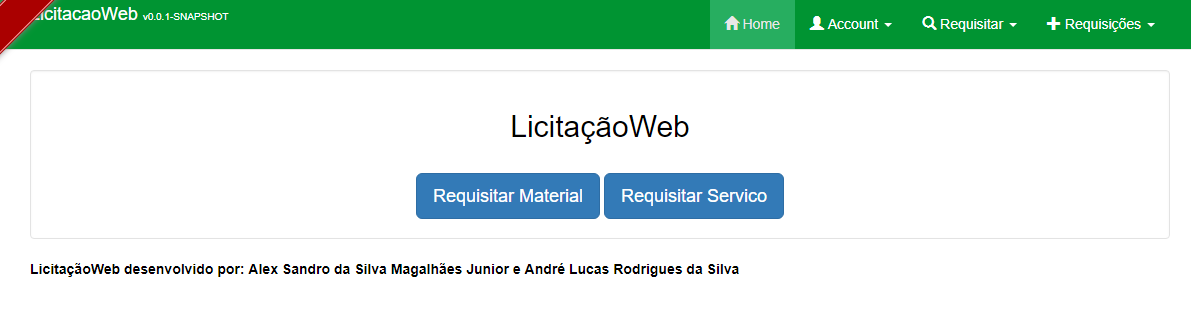
\includegraphics[width=0.75\textwidth]{figuras/prototipo001.png}
	\caption[PROT001: Tela home]{Tela inicial do sistema.}
	\label{tela01}
\end{figure}


\begin{figure}[htp]
	\centering
	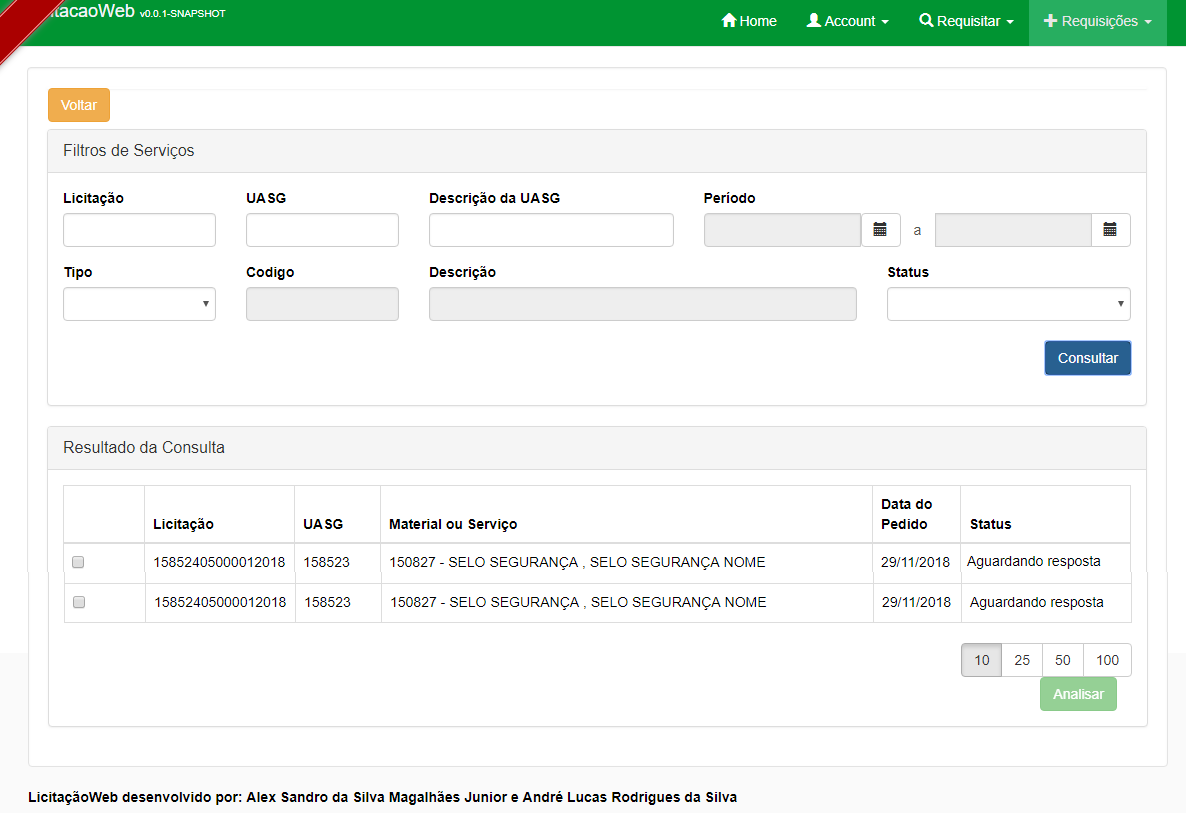
\includegraphics[width=0.75\textwidth]{figuras/prototipo006.png}
	\caption[Lista de Requisições]{Lista de requisições que cada ente recebe após iniciado um processo licitatório.}
	\label{tela02}
\end{figure}

\begin{figure}[htp]
	\centering
	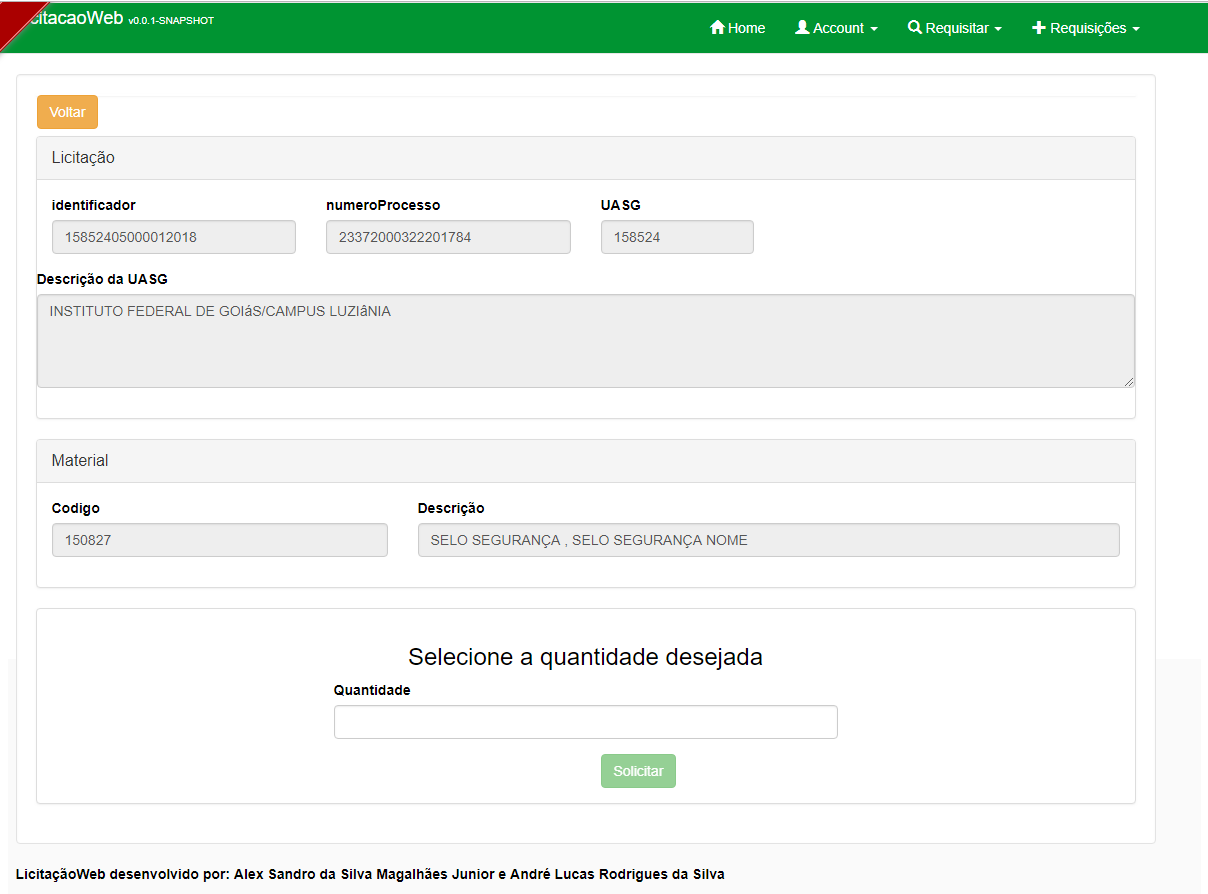
\includegraphics[width=0.75\textwidth]{figuras/prototipo003.png}
	\caption[Descrição do item selecionado]{Descrição da adesão de um ente ``B'' a um processo licitatório iniciado por um ente ``A'' para um item específico.}
	\label{tela03}
\end{figure}

\begin{figure}[htp]
	\centering
	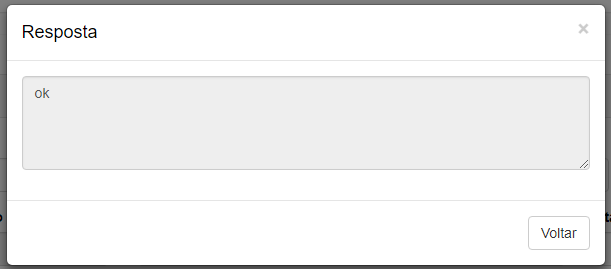
\includegraphics[width=0.75\textwidth]{figuras/prototipo010.png}
	\caption[Resposta da Requisição]{Resposta da requisição recebido pelo ente ``A'' após a adesão do ente ``B''.}
	\label{tela04}
\end{figure}


\section{Disponibilidade do Sistema}

Os sistema está disponível no GitHub, sob a Licença Apache 2.0, no endereço:
\begin{center}
	\url{https://github.com/dragao1995/licitacaoweb}
\end{center}




